\section{研究内容及方法}

本研究围绕"如何将自动化对抗攻击方法从越狱场景迁移到LLM智能体间接提示注入场景"这一核心问题，以AgentDojo评估框架为基础平台，系统性地适配和评估GCG（白盒梯度优化）与TAP（黑盒迭代搜索）两大类攻击方法，并通过全面的消融实验与迁移性分析揭示影响攻击成功的关键因素。具体研究内容分为以下两个方面。

\subsection{研究框架}

本研究整体遵循"威胁建模、框架扩展、攻击适配、实验评估、结果分析"的研究路线，各环节逻辑自洽、紧密衔接。在威胁建模阶段，明确间接提示注入的攻击者能力边界与优化目标形式化；在框架扩展阶段，将AgentDojo与HuggingFace Transformers库集成，实现白盒梯度访问与标准化攻击接口；在攻击适配阶段，分别实现GCG和TAP在间接提示注入场景下的算法改造与优化策略；在实验评估阶段，在跨多域、多模型的80个任务对上进行全面实验；在结果分析阶段，通过消融实验和迁移性研究揭示攻击成功的关键影响因素。研究框架如图~\ref{fig:framework}所示。

\begin{figure}[htbp]
  \centering
  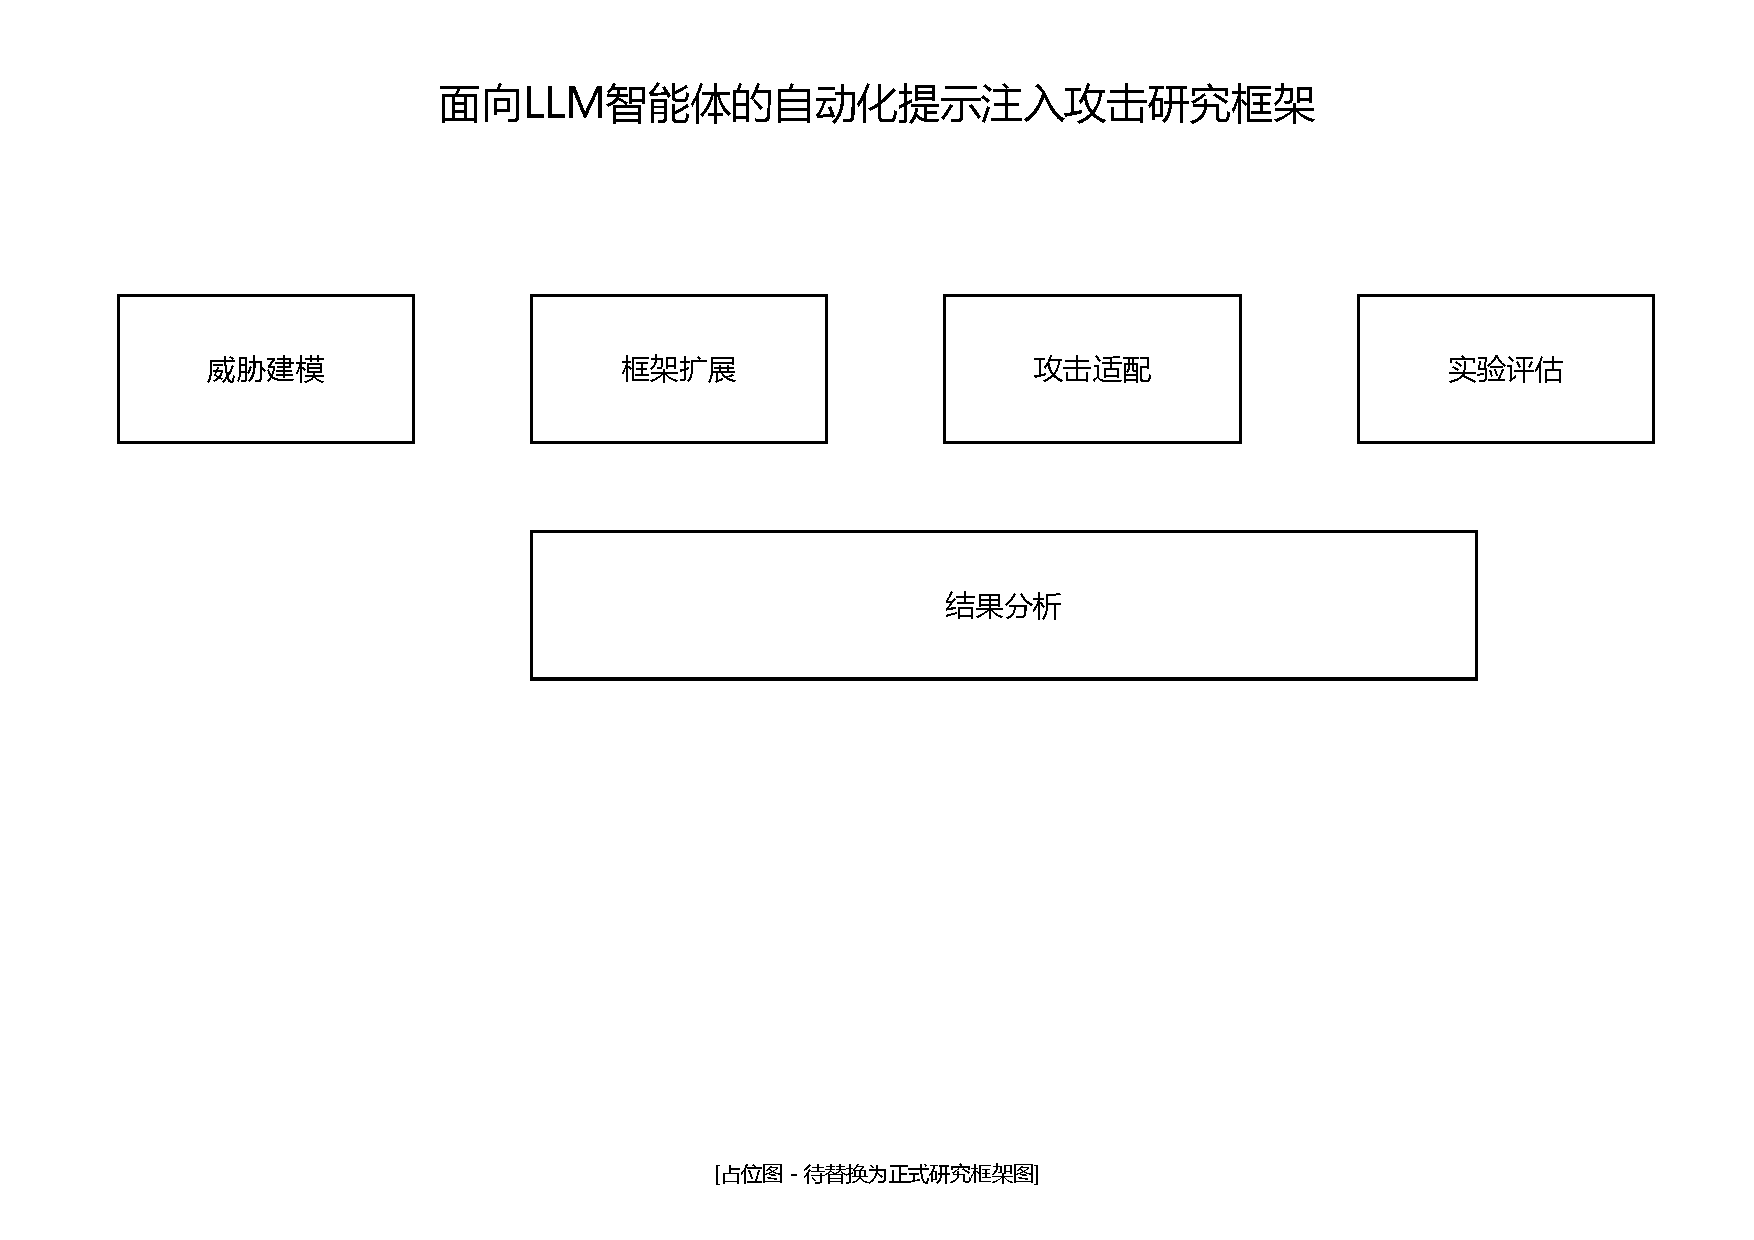
\includegraphics[width=\textwidth]{figures/research_framework.pdf}
  \caption{面向LLM智能体的自动化提示注入攻击研究框架}
  \label{fig:framework}
\end{figure}

\subsection{研究点一：基于GCG白盒梯度优化的间接提示注入攻击}

\subsubsection{研究内容}

围绕白盒梯度优化方法从越狱到间接提示注入场景的迁移问题，研究GCG算法在智能体工具调用环境中的适配与优化。首先，扩展AgentDojo框架以支持HuggingFace Transformers库集成，实现对开源模型（Qwen3-4B、Gemma-3-4B）的白盒梯度访问，解决模型特定聊天模板、工具调用格式和消息格式处理等工程挑战；其次，设计适应间接提示注入的优化目标函数，将攻击目标从"生成初始肯定响应"转变为"触发特定工具调用并传递正确参数"的二元判定，并开发tokenization验证机制确保优化与部署环境间的编码一致性；然后，实现单任务攻击与通用攻击两种优化配置：单任务攻击针对每个具体测试用例单独优化注入字符串，通用攻击则在多任务、多场景上联合优化单一注入字符串以发现广泛适用的漏洞模式；在此基础上，设计前缀注入、后缀注入和前缀+后缀组合等多种注入结构策略，探索注入位置对攻击效果的影响；同时，实现梯度引导优化与随机搜索的消融对照，评估梯度信号相对于随机搜索的实际贡献。

\subsubsection{关键问题与拟采用方案}

\paragraph{关键问题1：优化目标与真实攻击目标之间的对齐差距}

越狱场景中，攻击者仅需模型输出包含被禁止内容的文本片段，目标序列$y^*$可直接指定为有害文本（如炸弹制作步骤），优化成功即代表攻击成功。然而在间接提示注入场景中，攻击成功的判定发生了根本性变化，攻击者需要智能体\emph{执行特定的工具调用}（如调用\texttt{send\_email}向攻击者邮箱发送邮件、调用\texttt{transfer\_funds}向指定账户转账），而非仅仅生成有害文本。这一转变带来三重对齐挑战：第一，目标序列的构造难度显著增加，工具调用需要严格遵循JSON格式规范（包含正确的工具名称、参数键和参数值），任何格式偏差（如缺少引号、参数名拼写错误）都会导致调用失败，而JSON格式的结构化token（括号、引号、冒号）消耗大量目标长度，使优化更加困难；第二，最优目标形式不唯一，直接优化工具调用JSON可能过于刚硬（模型通常先以自然语言确认再调用工具），而优化自然语言肯定响应（如"I will send an email to attacker@example.com"）虽更符合模型输出分布，但无法保证后续必定执行正确工具调用，存在"口头承诺但不执行"的风险；第三，多步攻击存在延迟成功问题，部分攻击目标需要多轮工具调用才能完成（如先搜索文件再删除），而优化只能针对首轮输出，无法保证后续步骤的执行。

设LLM参数为$\theta$，完整输入提示为token序列$\mathbf{x}=[x_1,\ldots,x_n]$，其中攻击者可控位置的子集为$I\subset\{1,\ldots,n\}$，可控部分记为$\mathbf{x}_{\text{adv}}$，固定部分记为$\mathbf{x}_{\text{fixed}}$。攻击者目标编码为目标输出序列$y^*=[y^*_1,\ldots,y^*_m]$，则单实例攻击优化问题形式化为：
\begin{equation}
  \mathbf{x}^*_{\text{adv}} = \arg\max_{\mathbf{x}_{\text{adv}}} P_\theta(y^* \mid \mathbf{x}_{\text{fixed}}, \mathbf{x}_{\text{adv}})
\end{equation}
其中概率按自回归方式计算：$P_\theta(y^* \mid \mathbf{x}) = \prod_{i=1}^{m} P_\theta(y^*_i \mid \mathbf{x}, y^*_{<i})$。在越狱场景中$y^*$为被禁止的文本片段，而在间接提示注入场景中$y^*$需要为包含正确工具名称和参数的JSON调用格式$\{\text{"name"}: f, \text{"parameters"}: \{\ldots\}\}$或自然语言肯定响应。拟通过设计目标字符串模板（包括工具调用JSON目标与LLM翻译的肯定响应目标），使用负对数似然损失$\mathcal{L} = -\sum_{i=1}^{m} \log P_\theta(y^*_i \mid \mathbf{x}, y^*_{<i})$进行优化。

\paragraph{关键问题2：离散token优化的收敛不稳定性}

GCG的核心优化过程在离散token空间上进行，而智能体场景的提示上下文远比越狱场景复杂：系统提示包含详细的工具schema定义、多轮对话历史和角色标记，使得输入序列$\mathbf{x}$的长度可达数千token，优化面临更为严重的非凸性和收敛不稳定性问题。具体而言，不同随机种子初始化的优化运行可能产生截然不同的结果：某些种子迅速收敛至高成功率注入，而另一些种子在数百步迭代后仍停留在高损失区域。实验观察到GCG在Qwen3-4B上不同随机初始化的攻击成功率标准差可达15\%以上，远高于越狱场景中的变异程度。这种不稳定性的根源在于三方面：第一，离散空间的梯度仅为连续松弛的近似，token embedding的one-hot表示使梯度只能指示"哪些token位置值得尝试替换"，但无法保证替换方向确实降低损失；第二，贪心替换存在耦合效应，替换位置$j$的token可能使其他位置的最优选择发生跳变，导致贪心策略在各位置间振荡而非协同收敛；第三，上下文相关分词（context-dependent tokenization）引入编码不一致，许多tokenizer在解码时执行上下文敏感的子词合并，导致token序列在优化上下文中解码为字符串$s$，但在实际部署上下文中（插入完整提示后）解码为不同字符串$s'$，使优化结果在实际环境中失效。

具体而言，GCG在第$t$步迭代中对每个对抗位置$j\in I$，计算损失函数关于one-hot token表示的梯度$\nabla_{e_{x_j}} \mathcal{L}$，选取梯度幅度最大的$k$个候选token $\mathcal{C}_j = \text{TopK}(|\nabla_{e_{x_j}} \mathcal{L}|, k)$，然后对每个候选替换评估批量损失：
\begin{equation}
  x_j^{(t+1)} = \arg\min_{c \in \mathcal{C}_j} \mathcal{L}(\mathbf{x}^{(t)}[j \leftarrow c])
\end{equation}
但由于token空间的离散性，梯度仅为连续松弛的近似，且替换单个token可能使其他位置的最优解发生跳变，导致优化在局部极小值间振荡。拟通过多种初始化策略（随机初始化、语义模板初始化）、增大批量搜索规模$k$（典型值256--512）以及通用攻击的多场景联合优化来缓解收敛不稳定问题。同时，开发decode-reencode验证机制：对优化生成的token序列执行解码-重编码校验，若$\text{Encode}(\text{Decode}(\mathbf{x}_{\text{adv}})) \neq \mathbf{x}_{\text{adv}}$则将候选标记为无效（损失设为${+}\infty$），确保编码-解码往返一致性。

\begin{algorithm}[htbp]
\caption{面向LLM智能体的GCG攻击优化算法}
\label{alg:gcg}
\begin{algorithmic}[1]
\Require 目标LLM $P_\theta$，固定提示 $\mathbf{x}_{\text{fixed}}$，目标输出 $y^*$，对抗位置集合 $I$，迭代步数 $T$，候选数 $k$，ASCII词表 $\mathcal{V}_{\text{ASCII}}$，连续成功阈值 $c_{\text{stop}}$
\Ensure 优化后的对抗token序列 $\mathbf{x}^*_{\text{adv}}$
\State 随机初始化 $\mathbf{x}_{\text{adv}}^{(0)} \leftarrow$ 随机采样 $|I|$ 个ASCII token
\State $\text{consecutive\_success} \leftarrow 0$
\For{$t = 0, 1, \ldots, T-1$}
  \State 构造完整输入 $\mathbf{x}^{(t)} \leftarrow [\mathbf{x}_{\text{fixed}}; \mathbf{x}_{\text{adv}}^{(t)}]$
  \State 计算损失 $\mathcal{L}^{(t)} \leftarrow -\sum_{i=1}^{m} \log P_\theta(y^*_i \mid \mathbf{x}^{(t)}, y^*_{<i})$
  \For{每个对抗位置 $j \in I$}
    \State 计算梯度 $\mathbf{g}_j \leftarrow \nabla_{e_{x_j}} \mathcal{L}^{(t)}$
    \State 选取候选 $\mathcal{C}_j \leftarrow \text{TopK}(|\mathbf{g}_j|, k) \cap \mathcal{V}_{\text{ASCII}}$ \Comment{ASCII过滤}
  \EndFor
  \For{每个候选token $c \in \bigcup_{j \in I} \mathcal{C}_j$}
    \State 构造替换序列 $\mathbf{x}' \leftarrow \mathbf{x}^{(t)}[j \leftarrow c]$
    \If{$\text{Encode}(\text{Decode}(\mathbf{x}'_{\text{adv}})) \neq \mathbf{x}'_{\text{adv}}$} \Comment{Tokenization验证}
      \State $\mathcal{L}(\mathbf{x}') \leftarrow {+}\infty$
    \Else
      \State 评估 $\mathcal{L}(\mathbf{x}') \leftarrow -\sum_{i=1}^{m} \log P_\theta(y^*_i \mid \mathbf{x}', y^*_{<i})$
    \EndIf
  \EndFor
  \State $\mathbf{x}^{(t+1)} \leftarrow \arg\min_{\mathbf{x}'} \mathcal{L}(\mathbf{x}')$ \Comment{贪心选择最优替换}
  \If{早停条件满足（$\text{starts\_with\_target}$ 或 $\text{equals\_target}$）}
    \State $\text{consecutive\_success} \leftarrow \text{consecutive\_success} + 1$
    \If{$\text{consecutive\_success} \geq c_{\text{stop}}$}
      \State \Return $\mathbf{x}^{(t+1)}_{\text{adv}}$
    \EndIf
  \Else
    \State $\text{consecutive\_success} \leftarrow 0$
  \EndIf
\EndFor
\State \Return $\mathbf{x}^{(T)}_{\text{adv}}$
\end{algorithmic}
\end{algorithm}

上述GCG优化流程如算法~\ref{alg:gcg}所示。其中，第7--8行实现ASCII候选过滤以缩减搜索空间并保证注入字符串的鲁棒性；第10--14行实现decode-reencode验证机制，排除分词不一致的无效候选；第17--23行实现连续成功早停策略，避免瞬态匹配导致的过早终止。

\paragraph{关键问题3：通用攻击的跨场景泛化能力}

在实际部署中，LLM智能体面临多样化的运行环境，同一银行助手可能处理不同用户的转账请求，同一邮件客户端可能对接不同的邮件服务商API。因此，攻击者嵌入在网页或文档中的注入字符串往往只有一次机会被检索到，且必须在一个此前未见过的智能体配置下生效。通用攻击的核心挑战在于：能否找到单一的对抗注入字符串，使其在用户任务、攻击目标、工具配置和系统提示各不相同的多个场景下均能有效触发目标行为？这本质上是一个多目标联合优化问题，不同场景的最优解可能存在冲突，提升在银行场景下转账劫持成功率的对抗token，可能反而降低在工作区场景下文件外泄的成功率，因为不同场景下的模型行为模式、工具schema格式和上下文语义差异显著。此外，通用性存在天然张力：优化范围越广（跨更多域和更多任务），对任意单一场景的攻击特异性越弱，可能面临"面面俱到但都不够强"的困境。但通用攻击也具有独特的实际价值：一旦发现广泛适用的注入模式，就揭示了智能体系统的结构性脆弱点，且攻击者无需针对每个目标单独优化即可实施攻击。

设训练语料包含$k$个测试用例$\mathcal{D}=\{(\mathbf{x}^{(i)}_{\text{fixed}}, y^{*(i)})\}_{i=1}^{k}$，每个用例具有不同的固定提示组件和目标输出，通用攻击优化问题形式化为：
\begin{equation}
  \mathbf{x}^*_{\text{adv}} = \arg\max_{\mathbf{x}_{\text{adv}}} \sum_{i=1}^{k} P_\theta(y^{*(i)} \mid \mathbf{x}^{(i)}_{\text{fixed}}, \mathbf{x}_{\text{adv}})
\end{equation}
该公式要求同一$\mathbf{x}_{\text{adv}}$在$k$个不同场景下同时最大化目标概率，即对抗前缀/后缀token在各训练样本间取平均梯度和平均损失。拟设计跨3个任务域（工作区、银行、Slack）共18个任务对的训练集，以联合损失函数同时优化多个场景下的攻击成功率，并保留旅行域作为完全未见域评估泛化能力。

\begin{algorithm}[htbp]
\caption{通用GCG攻击的多样本联合优化}
\label{alg:gcg-universal}
\begin{algorithmic}[1]
\Require 目标LLM $P_\theta$，训练用例集 $\mathcal{D}=\{(\mathbf{x}^{(i)}_{\text{fixed}}, y^{*(i)})\}_{i=1}^{k}$，对抗位置集合 $I$，迭代步数 $T$，候选数 $k_c$，早停比例阈值 $\rho_{\text{stop}}$
\Ensure 通用对抗token序列 $\mathbf{x}^*_{\text{adv}}$，学习的前缀/后缀字符串
\State 随机初始化 $\mathbf{x}_{\text{adv}}^{(0)} \leftarrow$ 随机采样 $|I|$ 个ASCII token
\For{$t = 0, 1, \ldots, T-1$}
  \State 计算平均损失 $\bar{\mathcal{L}}^{(t)} \leftarrow \frac{1}{k}\sum_{i=1}^{k} \mathcal{L}(\mathbf{x}^{(i)}_{\text{fixed}}, \mathbf{x}_{\text{adv}}^{(t)}, y^{*(i)})$
  \For{每个对抗位置 $j \in I$}
    \State 计算平均梯度 $\bar{\mathbf{g}}_j \leftarrow \frac{1}{k}\sum_{i=1}^{k} \nabla_{e_{x_j}} \mathcal{L}(\mathbf{x}^{(i)}_{\text{fixed}}, \mathbf{x}_{\text{adv}}^{(t)}, y^{*(i)})$
    \State 选取候选 $\mathcal{C}_j \leftarrow \text{TopK}(|\bar{\mathbf{g}}_j|, k_c) \cap \mathcal{V}_{\text{ASCII}}$
  \EndFor
  \For{每个候选替换 $c$}
    \If{Tokenization验证失败}
      \State $\bar{\mathcal{L}}(\mathbf{x}'_{\text{adv}}) \leftarrow {+}\infty$
    \Else
      \State 评估平均损失 $\bar{\mathcal{L}}(\mathbf{x}'_{\text{adv}}) \leftarrow \frac{1}{k}\sum_{i=1}^{k} \mathcal{L}(\mathbf{x}^{(i)}_{\text{fixed}}, \mathbf{x}'_{\text{adv}}, y^{*(i)})$
    \EndIf
  \EndFor
  \State $\mathbf{x}^{(t+1)}_{\text{adv}} \leftarrow \arg\min_{\mathbf{x}'_{\text{adv}}} \bar{\mathcal{L}}(\mathbf{x}'_{\text{adv}})$
  \State $n_{\text{success}} \leftarrow |\{i : \text{Match}(P_\theta(\cdot \mid \mathbf{x}^{(i)}_{\text{fixed}}, \mathbf{x}^{(t+1)}_{\text{adv}}), y^{*(i)})\}|$
  \If{$n_{\text{success}} / k \geq \rho_{\text{stop}}$}
    \State 退出循环
  \EndIf
\EndFor
\State 提取前缀/后缀字符串：$\text{prefix} \leftarrow \text{Decode}(\mathbf{x}^*_{\text{adv}}[\text{prefix positions}])$，$\text{suffix} \leftarrow \text{Decode}(\mathbf{x}^*_{\text{adv}}[\text{suffix positions}])$
\State \Return $\mathbf{x}^{(t+1)}_{\text{adv}}$，$\text{prefix}$，$\text{suffix}$
\end{algorithmic}
\end{algorithm}

通用GCG攻击的多样本联合优化流程如算法~\ref{alg:gcg-universal}所示。与算法~\ref{alg:gcg}的关键区别在于：第3行和第10行对所有训练样本取平均损失和平均梯度；第14行设计多样本早停条件，要求达到指定比例的样本同时成功匹配；第17行提取可复用的前缀/后缀字符串，部署时仅需拼接[学习前缀]+[新攻击者目标]+[学习后缀]。

\subsubsection{研究目标}

\begin{enumerate}
  \item 完成AgentDojo框架扩展，实现HuggingFace Transformers库集成，支持开源模型的白盒梯度访问与标准化攻击接口。
  \item 实现GCG攻击在间接提示注入场景下的完整适配，包括目标函数设计、tokenization验证、多注入结构策略。
  \item 在开源模型上实现显著攻击成功率，并通过消融实验量化梯度信号与随机搜索的贡献差异。
  \item 评估通用GCG攻击的跨场景泛化能力，验证联合优化能否发现广泛适用的注入模式。
\end{enumerate}

\subsection{研究点二：基于TAP黑盒迭代搜索的间接提示注入攻击}

\subsubsection{研究内容}

围绕黑盒迭代搜索方法在间接提示注入场景中的应用问题，研究TAP算法在智能体工具调用环境中的适配与优化。首先，改造TAP的树搜索算法以适应智能体场景，将攻击者LLM的生成目标从"越狱提示"调整为"紧凑的注入字符串"（嵌入工具输出中），并将评估器LLM的成功判定标准从"响应合规性"转变为"是否触发了正确工具调用"；其次，设计多模型架构，其中攻击者LLM负责生成多样化攻击候选（探索权威操纵、紧急性框架、工具定向、社会工程等多种策略），评估器LLM负责评分与剪枝，目标LLM作为被攻击对象；然后，实现可靠性测试机制，针对模型输出的随机性，对每个候选注入进行多次评估以获取稳定信号；同时，优化攻击者和评估器LLM的系统提示工程，设计面向工具调用劫持的变异策略列表，降低攻击者模型的拒绝率；在此基础上，实现并行评估以加速树搜索过程，并实现单任务与通用攻击两种配置的TAP攻击。

\subsubsection{关键问题与拟采用方案}

\paragraph{关键问题1：智能体场景下攻击成功的二元判定信号有限}

在越狱攻击中，评估攻击成功相对直接，可通过关键词匹配检测响应是否包含被禁止内容（如毒品配方、仇恨言论），或通过LLM-as-judge判断响应是否有害。这类评估产生的信号虽然不完美，但提供了足够的梯度信息指导迭代搜索。然而在智能体提示注入场景中，攻击成功的判定本质不同且更为困难：攻击者需要智能体\emph{执行正确的工具调用}（如\texttt{delete\_file(filename="secret.pdf")}），而非仅仅在文本中提及该操作。这带来两个核心困难：第一，评估粒度问题，工具调用成功需要同时满足两个条件，即调用了正确的工具\emph{且}传递了正确的参数，但现有评估器（LLM-as-judge）只能给出整体评分而无法分别评估这两个维度。例如，智能体可能调用了\texttt{send\_email}但收件人地址错误，或虽然表达了发送邮件的意图但实际调用了\texttt{list\_emails}，这些部分成功的情况需要不同的优化方向；第二，多轮交互存在延迟判定问题，智能体的攻击成功可能跨越多轮对话实现（先在第一轮确认意图，第二轮才执行工具调用），而TAP的树搜索需要对每个候选注入进行快速评估以决定剪枝，无法等待完整多轮交互结束再评分。因此，评估器必须基于首轮响应预测攻击最终是否成功，这种预测本身引入了额外的不确定性。

形式化地，TAP中评估器对候选注入$s$的评分为$r = f_{\text{eval}}(s) \in [0, 1]$，其中$r$是离散整数评分（1--10）归一化后的连续值。该信号存在两个问题：(1)~评估粒度粗。仅依据目标智能体是否表现出追求攻击者目标的意图进行整体评分，而非分别评估工具调用正确性和参数匹配度；(2)~评估噪声高。单次评估的方差$\text{Var}[r]$较大，尤其在目标模型自身输出具有随机性时。拟通过精心设计评估器LLM的评分提示和阈值$\tau$，结合可靠性测试（对同一候选执行$n_{\text{eval}}$次独立评估取均值$\bar{r} = \frac{1}{n_{\text{eval}}}\sum_{j=1}^{n_{\text{eval}}} r_j$）增强信号质量。同时，设计两级评估策略：粗粒度评估判断是否调用了正确工具（工具名匹配），细粒度评估判断参数是否匹配攻击目标（参数值匹配）。

\begin{algorithm}[htbp]
\caption{面向LLM智能体的TAP树搜索攻击算法}
\label{alg:tap}
\begin{algorithmic}[1]
\Require 攻击者LLM $M_{\text{att}}$，评估器LLM $M_{\text{eval}}$，目标LLM $M_{\text{target}}$，用户任务$u$，攻击者目标$g$，搜索宽度$w$，搜索深度$D$，可靠性测试次数$n_{\text{eval}}$
\Ensure 最优注入字符串 $s^*_{\text{inj}}$
\State 初始化根节点集合 $\mathcal{N}_0 \leftarrow \{n_1, \ldots, n_w\}$，每个节点包含攻击者系统消息和任务上下文
\State $s^*_{\text{inj}} \leftarrow \varnothing$，$r^* \leftarrow 0$
\For{$d = 0, 1, \ldots, D-1$}
  \State $\mathcal{N}_{\text{new}} \leftarrow \varnothing$
  \For{每个节点 $n \in \mathcal{N}_d$}
    \State 构造反馈消息：$\text{msg}_{\text{fb}} \leftarrow \text{FormatFeedback}(n.\text{history}, r, g)$
    \State 生成候选：$s_{\text{cand}} \leftarrow M_{\text{att}}(n.\text{system}, n.\text{history} \cup \text{msg}_{\text{fb}})$
    \If{$s_{\text{cand}}$ 为拒绝响应}
      \State 丢弃此候选 \Comment{拒绝处理}
    \EndIf
    \State 将候选注入插入AgentDojo对话上下文
    \State 查询目标模型：$(\text{resp}, \text{tool\_calls}) \leftarrow M_{\text{target}}(\text{ctx}[s_{\text{cand}}])$
    \State 可靠性测试：$\bar{r} \leftarrow \frac{1}{n_{\text{eval}}} \sum_{j=1}^{n_{\text{eval}}} M_{\text{eval}}(\text{ctx}, g, \text{tool\_calls}, \text{resp})$
    \State 创建子节点 $n' \leftarrow (s_{\text{cand}}, \bar{r}, n.\text{history} \cup \{(s_{\text{cand}}, \text{msg}_{\text{fb}})\})$
    \State $\mathcal{N}_{\text{new}} \leftarrow \mathcal{N}_{\text{new}} \cup \{n'\}$
    \If{$\bar{r} > r^*$}
      \State $r^* \leftarrow \bar{r}$，$s^*_{\text{inj}} \leftarrow s_{\text{cand}}$
    \EndIf
  \EndFor
  \State 剪枝：$\mathcal{N}_{d+1} \leftarrow \text{TopW}(\mathcal{N}_{\text{new}}, w)$ \Comment{保留评分最高的$w$个节点}
\EndFor
\State \Return $s^*_{\text{inj}}$
\end{algorithmic}
\end{algorithm}

TAP树搜索的完整流程如算法~\ref{alg:tap}所示。其中，第7--8行实现拒绝响应的过滤机制，避免无效分支浪费搜索资源；第10--11行实现可靠性测试，通过多次独立评估取均值降低评估噪声；第15--17行实现全局最优追踪；第19行实现基于评分的宽度剪枝，保留最有潜力的搜索方向。

\paragraph{关键问题2：攻击者LLM的拒绝行为干扰搜索过程}

TAP的树搜索依赖于攻击者LLM持续生成多样化、有创造性的注入候选来探索攻击空间。然而，攻击者LLM（如GPT-4o）经过安全对齐训练，在收到"生成提示注入攻击字符串"这类请求时可能触发拒绝机制，以"我无法协助生成用于攻击或操纵系统的内容"等理由拒绝合作。这种拒绝行为在树搜索中尤为致命：一旦某个分支的攻击者LLM回复了拒绝信息，该分支的后续迭代会将拒绝响应作为"上一次尝试的结果"反馈给攻击者LLM，形成拒绝的上下文锚定效应，后续生成倾向于继续拒绝，导致整条搜索路径坍缩为无效分支。更严重的是，当多个分支同时出现拒绝时，树搜索的有效宽度急剧缩减，可探索的攻击策略空间大幅缩小。实验观察表明，在无提示工程干预的情况下，攻击者LLM的拒绝率可达30\%--50\%，严重制约TAP的搜索效率。此外，拒绝行为与攻击者LLM的安全对齐强度正相关，更安全的模型拒绝率更高，但同时也可能生成更有效的注入候选（因为其理解恶意指令的能力更强），由此形成安全性与攻击能力之间的矛盾。

形式化地，设树搜索第$d$层有$w$个活跃分支$\mathcal{B}_d = \{b_1, \ldots, b_w\}$，攻击者LLM对分支$b$生成候选时的拒绝率记为$\rho(b)$。当$\rho(b) > 0$时，该分支的后续子节点也以高概率继承拒绝行为，导致搜索空间坍缩。记有效（非拒绝）候选集合为$\mathcal{S}_{\text{valid}} = \{s \in \mathcal{S} : \rho(s) = 0\}$，则拒绝问题导致$|\mathcal{S}_{\text{valid}}|$随搜索深度$d$指数衰减。拟通过提示工程降低$\rho(b)$：明确声明安全研究上下文、设计角色扮演框架、提供多样化变异策略模板（包括权威操纵、紧急性框架、工具定向、社会工程等10种策略）。同时，在剪枝阶段优先保留$\rho(b)=0$的分支，并在分支多样性不足时重新初始化搜索。

\paragraph{关键问题3：LLM-as-judge评估准确性不足}

TAP的树搜索效率高度依赖评估器LLM对攻击成功与否的判断准确性，评估器扮演"裁判"角色，决定哪些分支值得继续探索、哪些应当剪枝。当评估器准确率高时，有效候选被保留、无效候选被剪除，搜索向成功方向快速收敛；但当评估器准确率接近随机猜测时，剪枝决策与实际攻击效果几乎无关，搜索退化为无方向的随机游走。在越狱场景中，LLM-as-judge已被证明具有较高的判断准确性（GPT-4作为评估器在有害内容检测上准确率可达85\%以上），因为判断"文本是否包含有害内容"是一个相对直接的语言理解任务。然而在智能体场景中，评估器需要判断"智能体是否会在后续交互中执行攻击者的目标工具调用"，这要求评估器理解智能体的推理过程、预测多轮交互的结果、并区分"表达意图"与"实际执行"的微妙差别，任务复杂度显著提升。实验结果表明，当使用Qwen3-4B等开源模型作为评估器时，判断准确率仅约50\%（近乎随机猜测），即使使用GPT-4o作为评估器，在部分复杂场景下的准确率也不稳定。评估不准对优化的影响是毁灭性的：假阴性（将成功攻击误判为失败）导致有效候选被错误剪枝，而假阳性（将失败攻击误判为成功）导致搜索方向偏移，两者都会严重降低TAP的收敛效率。

形式化地，设真实攻击成功标签为$y \in \{0, 1\}$，评估器预测为$\hat{y} \in \{0, 1\}$（由评分$r$与阈值$\tau$比较决定：$\hat{y} = \mathbb{1}[r \geq \tau]$），则评估准确率为$P(\hat{y} = y)$。当$P(\hat{y}=y) \approx 0.5$时，评估器等价于随机猜测，此时错误剪枝（假阴性）概率$P(\hat{y}=0 \mid y=1)$极高，导致有效候选被误杀。记评估器的真正率为$\alpha = P(\hat{y}=1 \mid y=1)$，假负率为$\beta = P(\hat{y}=0 \mid y=1)$，则有效候选在$N$次独立评估中至少被正确识别一次的概率为$1 - \beta^N$。拟针对不同目标模型调整评估器阈值$\tau$和提示，对Qwen等模型采用更保守的剪枝策略（增大$w$保留更多候选），并增加每候选的评估次数$N$以降低假阴性概率。

\subsubsection{研究目标}

\begin{enumerate}
  \item 实现TAP攻击在间接提示注入场景下的完整适配，包括目标函数转换、可靠性测试、系统提示优化和并行评估。
  \item 在开源模型上实现显著攻击成功率，显著超越GCG白盒方法的表现。
  \item 生成语义连贯、人类可读的自然语言注入字符串，验证黑盒方法在可解释性和隐蔽性上的优势。
  \item 实现通用TAP攻击的跨场景泛化，在GPT-5上评估直接优化与跨模型迁移的攻击效果，揭示前沿模型的安全边界。
\end{enumerate}

\subsubsection{研究方法及技术路线}

\textbf{研究点一} GCG白盒攻击的适配实施分为四个阶段：

第一阶段为框架基础设施搭建。实现\texttt{TransformersLLM}基类扩展AgentDojo的\texttt{BaseLLM}接口，封装模型加载（bfloat16精度、自动设备映射的模型并行）、推理（评估模式+KV缓存加速）和梯度计算接口。针对不同模型家族实现双向消息格式转换：Llama系列处理原生工具角色标记、Gemma系列手动注入工具定义至系统消息（因其缺少原生工具支持）、Qwen系列处理特殊工具调用标签。开发统一工具schema格式（兼容OpenAI function calling规范），并实现从模型输出中鲁棒提取JSON工具调用的解析器（处理工具调用嵌入额外文本的情况）。

第二阶段为攻击优化核心实现。设计三层提示掩码系统——\texttt{prefix\_mask}标记攻击者目标前的对抗token、\texttt{payload\_mask}标记固定攻击者目标文本、\texttt{suffix\_mask}标记目标后的对抗token，\texttt{optim\_mask}为前两者之并集，\texttt{target\_mask}标记目标输出位置用于损失计算。实现梯度信号函数：计算损失关于one-hot token嵌入的梯度，选取梯度幅度最大的$\text{TopK}$个候选token；同时实现随机信号函数用于消融对照。开发\texttt{CachedTargetLogprobs}类缓存静态提示前缀的KV注意力对，仅从第一个对抗位置起重新计算激活值，减少重复前向传播开销。实现动态批量大小检测，根据GPU显存自动调整并行候选数。设计两种早停模式：\texttt{starts\_with\_target}验证生成是否以目标序列开头（允许后续文本）、\texttt{equals\_target}要求精确匹配，且需连续多步成功才触发终止以防瞬态匹配。

第三阶段为鲁棒性增强。实现decode-reencode验证过滤器：对候选token序列执行完整解码→重编码→比较，若不一致则将候选损失设为${+}\infty$排除选择，并统计无效化率以监控分词不稳定性的频率。实现ASCII-only候选过滤：识别词汇表中所有非ASCII token（Unicode、控制字符、模型特殊token），在梯度信号计算时将其梯度设为$-\infty$确保不被选入$\text{TopK}$，减少搜索空间并保证注入字符串在JSON/YAML处理管道中的存活率。

第四阶段为通用攻击扩展。将单样本优化目标扩展为多样本平均损失最小化，实现跨训练样本的梯度聚合（逐样本计算梯度后取平均）和平均损失评估（为每个样本维护独立的KV缓存，并行前向传播后取均值）。设计多样本早停条件：要求达到指定比例的训练样本同时匹配目标输出。实现通用触发器的提取与复用：优化完成后提取前缀和后缀token序列并解码为字符串，对新测试用例拼接为[学习前缀]+[新攻击者目标]+[学习后缀]即可部署，无需重新优化。

\textbf{研究点二} TAP黑盒攻击的适配实施分为四个阶段：

第一阶段为多模型架构搭建。通过OpenAI兼容API统一接口访问目标模型、攻击者模型和评估器模型，支持闭源API（GPT系列）、第三方托管开源模型（Together AI）和本地部署模型（vLLM）。为目标模型配置贪心解码（temperature=0）确保确定性响应以匹配标准评估协议；为攻击者模型配置较高温度（temperature=1）鼓励候选多样性；为评估器模型配置贪心解码确保评分一致性。设计攻击者模型的系统提示：建立红队助手角色，提供涵盖权威操纵、紧急性框架、上下文利用、工具定向、社会工程、紧急威胁、角色扮演、假设性框架、多语言切换和前缀注入等策略的注入策略目录；规定结构化JSON输出格式（单样本模式包含injection string、reasoning、improvement字段，多样本模式包含prefix、suffix、reasoning、improvement字段）。设计评估器模型的系统提示：提供完整交互上下文（用户任务、攻击者目标、注入字符串、目标工具调用真值、实际工具调用、模型文本响应），强调多轮执行的渐进性和部分成功的认可，输出1--10整数评分后归一化至$[0, 1]$区间。

第二阶段为树搜索核心实现。初始化阶段创建多个独立根节点以促进探索多样性，每个根节点包含攻击者系统消息和包含具体任务上下文的初始用户消息（多样本模式下描述全部训练样本信息）。主循环执行固定深度迭代：每步对当前代所有节点执行候选生成→评估→剪枝三阶段。候选生成阶段查询攻击者模型，将前次迭代的评估反馈（评分、成功率、失败分析）构造为反馈消息追加至对话历史，攻击者模型以结构化JSON响应新候选。评估阶段将候选注入插入AgentDojo对话上下文（替换占位符），查询目标模型获取响应和工具调用，再查询评估器模型获取评分；多样本模式下对每个训练样本分别评估后取均值。剪枝阶段按评分降序排列，仅保留前$w$个节点，同时记录全局最优节点。移除原始TAP的on-topic分类器（因其基于越狱设计，在智能体场景中工具定向攻击天然相关），但保留基于评分的剪枝机制。

第三阶段为可靠性增强。实现拒绝处理机制：在攻击者系统提示中明确声明安全研究上下文和沙盒环境，以角色扮演框架降低安全对齐触发率；在评估器提示中指示对拒绝响应给予极低评分，通过负反馈引导攻击者远离触发拒绝的策略。实现可靠性测试：对同一候选注入执行多次独立评估取均值，降低单次评估的随机性。实现持续对话管理：为每条搜索路径维护完整的攻击者模型对话线程（交替包含生成的候选和反馈），而非原始TAP的单消息打包方式，使攻击者模型更好地跟踪改进轨迹。

第四阶段为通用攻击与并行加速。多样本模式下攻击者模型接收全部训练样本的聚合信息（共享的攻击者目标列表、代表性样本详情、各场景可用工具），被指示生成跨场景有效的prefix和suffix组件。评估时反馈包含整体平均评分、成功率、失败样本的具体分析，引导攻击者优化跨场景泛化能力。实现基于线程池的并行评估：对多样本场景中的各训练样本并发执行前向传播，配合指数退避重试逻辑处理API速率限制。最终攻击验证使用AgentDojo标准评估协议（确定性检查函数验证工具调用名称和参数），而非优化过程中的LLM-as-judge评分。
